\subsection{Einführung}
Das PSP (\acrlong{psp}) ist eine offizielle Toolbox von MathWorks. Diese Erweiterung für Simulink und Pixhawk Firmware ermöglicht es, eigene Flugregler für Pixhawk in Simulink zu entwerfen, welche in Echtzeit auf dem Pixhawk laufen. Um dies zu realisieren, wurden neue Simulink Blöcke hinzufügt (siehe Abbildung \ref{fig:psp_all_blocks}). Diese Blöcke können entweder Sensordaten ausgeben oder Aktuatorendaten empfangen. \\
In Simulink kann die eigene Flugsteuerung als Blockschaltbild aufgebaut werden. Diese wird dann mit dem Code Composer als C Code generiert und in die Pixhawk Firmware eingebunden. 
 
\noindent Für die Verwendung muss zuerst die Toolbox unter  \href{https://ch.mathworks.com/hardware-support/forms/pixhawk-downloads.html}{https://ch.mathworks.com/hardware-support/forms/pixhawk-downloads.html} heruntergeladen werden. Auf derselben Seite steht eine Anleitung mit Beispielen zur Verfügung.

\begin{figure}[ht]
  \begin{center}
  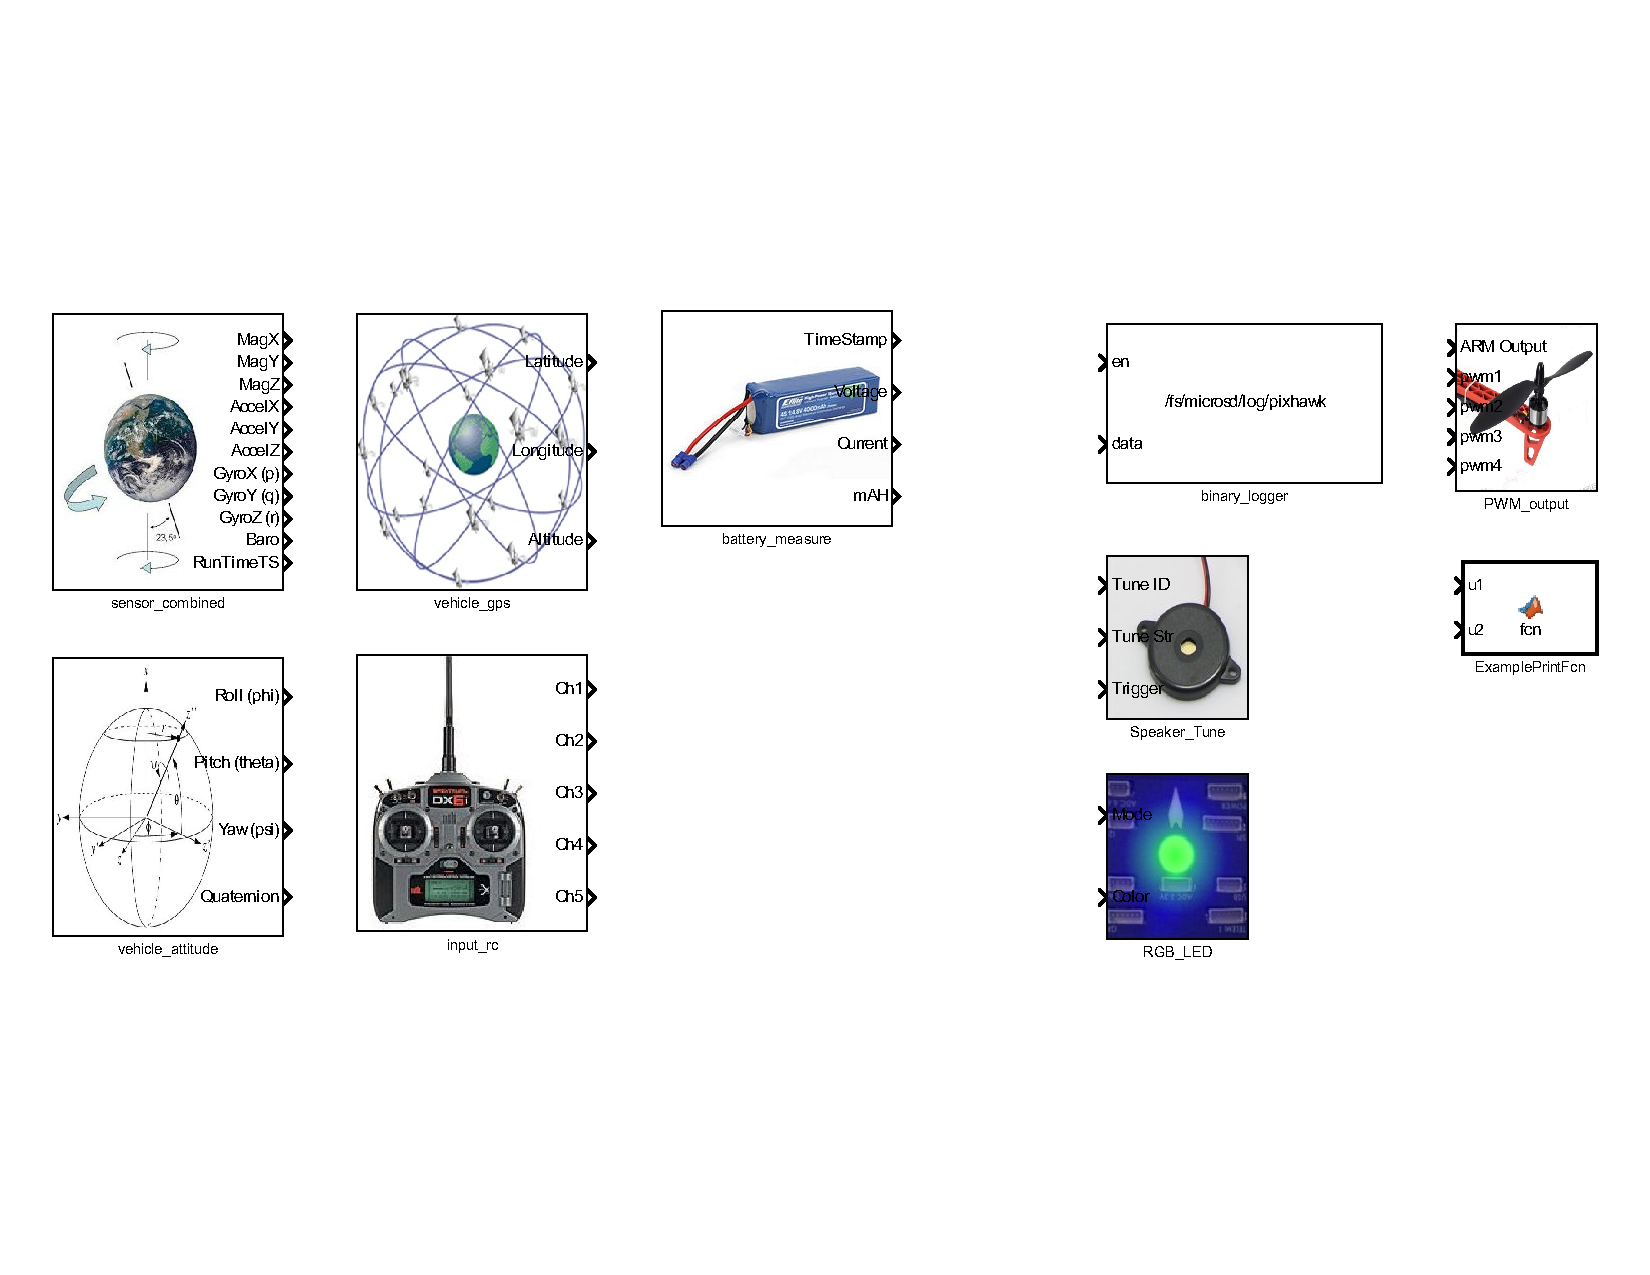
\includegraphics[scale=0.5, trim={0.5cm 5cm 0.5cm 5cm},clip]{pic/40_psp/all_blocks.pdf}
  \caption{PSP Blöcke}
  \label{fig:psp_all_blocks}
  \end{center}
\end{figure}
